\section{Program Elements with Documentation Comments} 
The rule of thumb is that every program element that got a name requires a documentation comment. The exceptions are local variables\footnote{but refer to chapter \tqfullref{sec:LocalVariableComments}.} and labels\index{label}.

This means that we have documentations comments for
\begin{itemize}[nosep]
	\item{modules}
	\item{packages}
	\item{classes\index{class}, interfaces\index{interface}, records\index{record}, \lstinline|enum|s\index{enum} and annotations\index{annotation}}
	\item{methods\index{method} and constructors\index{constructor}}
	\item{parameters and record\index{record} components}
	\item{fields (attributes and constants) and \lstinline|enum|\index{enum} values}
\end{itemize}

In addition, Javadoc\index{javadoc} allows you to generate a project overview as part of the documentation. The source for this is an HTML file that is typically stored outside the source tree. For the details, see the chapter \hyperref[sec:OverviewDoc]{below}.

%------------------------------------------------------------------------------

\subsection{The \bsq{Overview}}\label{sec:OverviewDoc}
The Overview page is not a typical documentation comment; its source is an HTML\index{HTML} document that is referenced through the command line option \mbox{\bsq{\texttt{-overview}}} (see \tqfullvref{sec:Locations} and \autocite{ORACLE_DOC_JAVADOC_MAN:StandardDocletOptions}) when the Javadoc tool\index{javadoc} is called to generate the documentation for your project. It takes the the (fully-qualified) name of that file as the argument; the recommended filename is \bdq{\texttt{overview.html}}.

The file itself should be a valid HTML~5\index{HTML} document; you can omit the \lstinline|<head>| section because the Javadoc\index{javadoc} will copy only a section \lstinline|<main>| into the generated documentation, or, if this does not exist, the whole \lstinline|<body>| section.

Several Javadoc\index{javadoc} tags can be also used in the overview document; for details refer to the section \bdq{Where Tags Can Be Used}in \autocite{ORACLE_DOC_JAVADOC_TAG}.

The content of that overview can be nearly everything, from the project's history through build or installation instructions to the manual on how to use the program or library that is delivered through the project. However, you should not duplicate information that is in the module, package, or class documentation comments. If important, you can set reference links to these.

Since Java~23, the overview document can be also a Markdown\index{Markdown} document (see \autocite{JEP467,ORACLE_DOC_JAVADOC_GUIDE:Markdown}); in that case, the recommended file name would be\linebreak \bdq{\texttt{overview.md}}. 

%==============================================================================
% End of file!!
%==============================================================================


\subsection{The \bsq{module} Comment}\label{sec:ModuleComment}
The documentation comment for a module is part of the \texttt{module-info.java} file for that module (refer to chapter \tqfullref{sec:ModuleDefinition}).

The \texttt{<module description>} is regular documentation comment, followed by the mdoule definition. It describes the module, its dependencies and what it provides. See the Javadoc\index{javadoc} tags \bdq{\nameref{sec:TagProvides}}\index{provides@"@provides} and \bdq{\nameref{sec:TagUses}}\index{uses@"@uses} for details.

The module documentation comment should not list the packages; this will be done automatically through the Javadoc\index{javadoc} tool during the generation process. Is should also not describe the packages; this is part of the package documentation.
 
If the project has just one module, the module comment can replace the overview comment (see \hyperref[sec:OverviewDoc]{above}).

%==============================================================================
% End of file!!
%==============================================================================


\subsection{The ‘package’ Comment}\label{sec:PackageComment}
The documentation comment for a package\index{package} lives in a dedicated file, the \texttt{package-info.java}\index{package-info.java}, that exists mainly for that comment; refer to \tqfullvref{sec:PackageDocumentation}.

Such a file has to be there for each Java package\index{package}.

The \texttt{<package description>} should provide information about the package\index{package}. It describes the purpose of the classes\index{class} within this package\index{package} without, however, going into detail about individual classes – that is reserved for the documentation comment of the class\index{class} itself.

Furthermore, it contains conventions that applies equally to all classes\index{class} of the package\index{package}; for instance, the package\index{package} description often includes statements such as: \bdq{For all methods\index{method} in this package\index{package}, \lstinline|null| is not permitted as an argument unless explicitly stated otherwise in the documentation for the specific method\index{method}.}

If the package\index{package} defines a single API, it can describe the usage of that API, too. 

The package comment can list the authors of the code, using the \bdq{\nameref{sec:TagAuthor}}\index{author@"@author} tag, the version with the \bdq{\nameref{sec:TagVersion}}\index{version@"@version} tag, the date when the package\index{package} was created or with which version it was integrated, using the \bdq{\nameref{sec:TagSince}}\index{since@"@since} tag, and other things.

It should not repeat details that are written already in the documentation of a class\index{class} in that package, instead it should reference that class documentation. If those details are  important for the whole package, it should be considered to move them from the class comment to the package description and place a reference into the class documentation instead.

The package comment for the main package\index{package!main package} of a project can replace the \hyperref[sec:OverviewDoc]{overview comment} (if not the \hyperref[sec:ModuleComment]{module comment} is used for this\footnote{Not all projects will produce modules, so it is possible that your project does not have a module definition file at all.}).

%==============================================================================
% End of file!!
%==============================================================================


\subsection{The ‘class’ Comment}\label{sec:ClassComment}
The documentation comment for a class\index{class}, an interface\index{interface}, an \lstinline|enum|\index{enum}, a record\index{record} or an annotation\index{annotation} (the \bsq{class comment}) describes that class, its purpose and its usage. If the class is not \lstinline|final|, the comment should provide some hints what the mount points\index{mount point}\footnote{Another term for \bdq{mount point} is \bdq{extension point}\index{extension point|see {mount point}}, but I do not like this expression as we do not always \textit{extend} a class on these points. Most often we replace existing behaviour to customise the class to our needs.} are and how to utilise them.

Then the class comment should list the authors of the class, using the \nameref{sec:TagAuthor}\index{author@"@author} tag, the class version (using the \nameref{sec:TagVersion}\index{version@"@version} tag), and when the class was added to the project with the \nameref{sec:TagSince}\index{since@"@since} tag, although this is optional if the information is already given within the package comment.

In case of a parameterized type\index{parameterized type} (a \bsq{generic}), the class comment must contain a \nameref{sec:TagParam}\index{param@"@param} tag for each formal parameter.

\keeplisting{17}
Here a real life sample for an interface\index{interface}
\begin{lstlisting}
/**
 *  <p>{@summary This is the basic interface for any kind of DAO 
 *  (Data Access Object).} It is based on sample code from the book 
 *  &quot;Java Persistence with Hibernate&quot;.</p>
 *
 *  @param  <T> The entity type for the DAO.
 *  @param  <I> The type of the entity id.
 *
 *  @author Thomas Thrien - thomas.thrien@tquadrat.org
 *  @version 2.3.4
 *  @since 1.2.3
 */
public interface GenericDAO<T,I>
{
    …
}   //  interface GenericDAO
\end{lstlisting}

The version information for the \nameref{sec:TagVersion}\index{version@"@version} tag (line~10) should be a reference to the version in the SCCS\index{SCCS}; if you are using Subversion\index{Subversion}, that line would look like this:
\begin{lstlisting}[firstnumber=9,language=Comment]
 …
 *  @version $Id:$
 …
\end{lstlisting}

The string \verb#$Id:$# will be replaced during checkin with information provided by Subversion\index{Subversion} if \bdq{\textit{keyword replacement}} is enabled. git\index{git} does not provide something similar out-of-the-box.

The class comment for a record\index{record} is a bit special as it has to incorporate the documentation for the record components (the fields of the record) as well as that for the constructor parameters (as both are the same). You use the \nameref{sec:TagParam}\index{param@"@param} tag for that.

The declaration for a record\index{record} \lstinline|Tupel| is shown below. Although not explicitly declared, the record\index{record} class has~…
\begin{itemize}[nosep]
	\item{…~a constructor\index{constructor}:
\keeplisting{4}
\begin{lstlisting}
public Tupel( final K key, final V value )
{
    this.key = key;
    this.value = value;
}
\end{lstlisting}}

	\item{…~the two attributes \bdq{\lstinline|public final K key|} and \bdq{\lstinline|public final V value|}}

	\item{
	\keeplisting{2}
	…~the two accessor methods\index{method!accessor method}:
\begin{lstlisting}
public final K key() { return key; }
public final V value() { return value; }
\end{lstlisting}}

	\item{…~and implementations for the methods \bdq{\lstinline|equals()|}, \bdq{\lstinline|hashCode()|} and \bdq{\lstinline|toString()|}}
\end{itemize}

The documentation for these elements is generated either based on the arguments for the \nameref{sec:TagParam} tags (see lines~13 and 14) or from standard texts.

\begin{lstlisting}[caption={A tupel class}]
/**
 *  <p>{@summary A tupel.} The first entry, usually referred to as 
 *  the &quot;key&quot; identifies the object, the second one is the
 *  &quot;value&quot;.</p>
 *  <p>The sort order is determined only through the keys, therefore
 *  {@link #compareTo(Tupel)}
 *  is not consistent with
 *  {@link #equals(Object)}.</p>
 *
 *  @param  <K> The type of the key.
 *  @param  <V> The type of the value.
 *
 *  @param  key The key of the tupel; can be {@code null}.
 *  @param  value   The value of the tupel; can be {@code null}.
 *
 *  @author Thomas Thrien - thomas.thrien@tquadrat.org
 *  @version $Id:$
 *  @since 1.2.3
 */
public record Tupel<K extends Comparable<K>,V>( K key, V value ) implements Comparable<Tupel<K,V>>
{
        /*---------*\
    ====** Methods **================================================
        \*---------*/
    /**
     *  {@inheritDoc} 
     */
    @Override
    public final int compareTo( final Tupel<K,V> o )
    {
        final var retValue = Comparator.comparing( Tupel<K,V>::key )
            .compare( this, o ); 

        //---* Done *------------------------------------------------
        return retValue;
    }   //  compareTo()
}
//  record Tupel
\end{lstlisting}
\clearpage
This is the first part of the class documentation, generated by the Javadoc\index{javadoc} tool from the source code above:
\begin{center}
	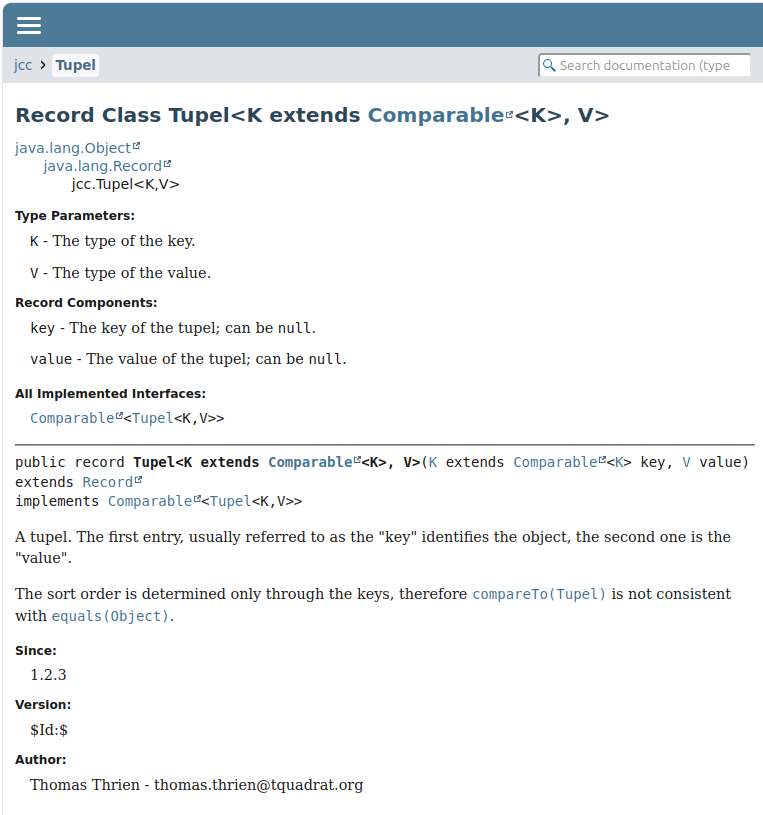
\includegraphics[scale=0.55]{comments/JavadocTupel1}
\end{center}

\clearpage
Despite none of the methods\index{method} nor the constructor\index{constructor} were explicitly defined, they are listed for the \lstinline|Tupel| record class\index{record}, even with a meaningful description:
\begin{center}
	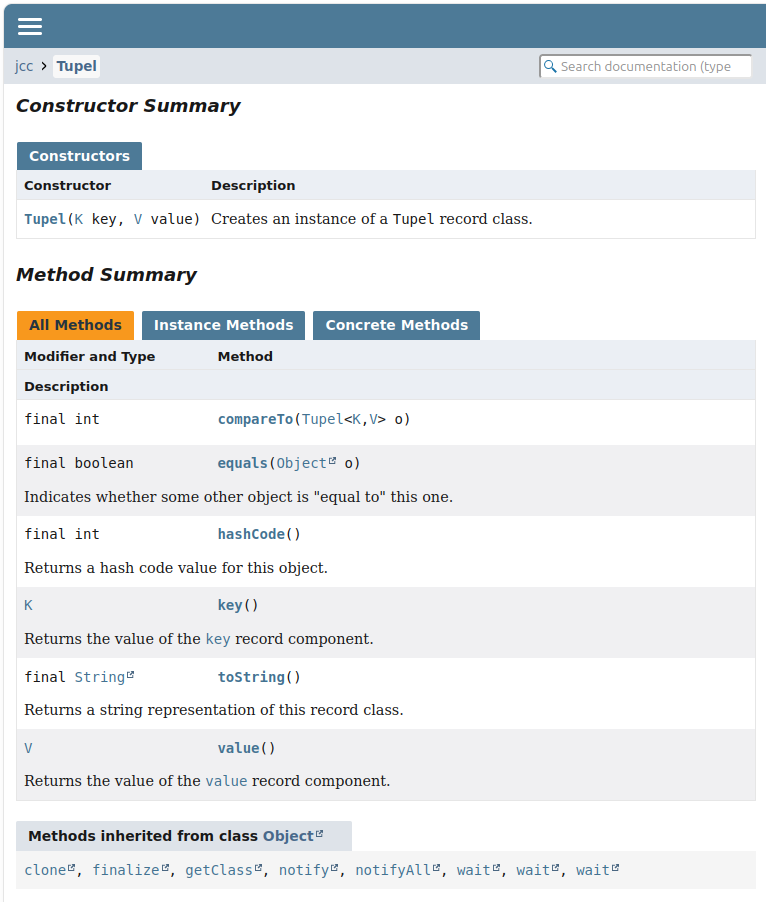
\includegraphics[scale=0.55]{comments/JavadocTupel2}
\end{center}
That there is no description for \lstinline|compareTo()| is due to a bug in the Javadoc tool in the version used for the generation; usually, the documentation is inherited from the overridden method\index{method!overridden method}. At the very least, the Javadoc tool\index{javadoc} generated the link to the documentation of the overridden method\index{method!overridden method} within the method's detailed documentation:
\begin{center}
	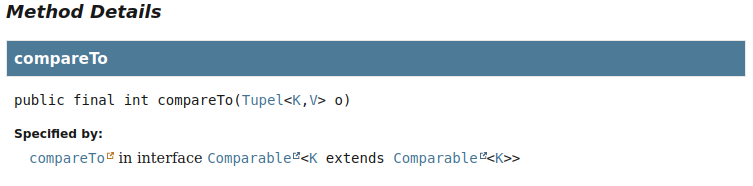
\includegraphics[scale=0.55]{comments/JavadocTupel3}
\end{center}

%==============================================================================
% End of file!!
%==============================================================================

\subsection{The Field Comment}\label{sec:FieldComment}
Attributes/properties\index{field!attribute}\index{property}, constants\index{field!constant} and \lstinline|enum|\index{enum} values are all summarised under \bsq{field}\index{field} here.

Each and every field\index{field} must have a comment, the \bsq{field comment}, describing it. For private fields\index{field} it can be sufficient to refer to the related getter method\index{method!getter method}\footnote{Of course you have to provide a complete documentation of the property\index{property} there; just a line with a \bdq{\{\nameref{sec:TagReturn} …\}}\index{return@"@return} inline tag will not do the job for the getter method\index{method!getter method} in this case.} instead of writing a lengthy comment into the field comment itself; but do not use the \bdq{\nameref{sec:TagSee}}\index{see@"@see} tag instead of the \bdq{\{\nameref{sec:TagLink} …\}}\index{link@"@link} tag:
\begin{lstlisting}
/**
 *  <p>{@summary For the description of the property 'value' refer to
 *  {@link #getValue()}.
 */
private final Value m_Value;

// AVOID!! Do not use @see
/**
 *  @see #getOtherValue()}.
 */
private final Value m_OtherValue;
\end{lstlisting}

If there is no getter method\index{method!getter method} for the field\index{field}, or if it is not private, a proper description is mandatory. One sentence is enough in most cases, but you are not limited to that.

It is always a good idea to describe the valid values for the field\index{field}, its default value, and whether \lstinline|null| is a possible value for a reference. This is a hard requirement for all non-final non-private fields\index{field} – in particular because there should \textit{never} be any non-final non-private fields\index{field} at all!

For a serialisable class\index{class}\index{serialization}, the fields\index{field} that will be serialised should be tagged with \bdq{\nameref{sec:TagSerial}}\index{serial@"@serial} and the appropriate description.

% Elaborate on comments for constants!!!!





Constants (\lstinline|public static final| fields) that are initialised with a literal have to use the \nameref{sec:TagValue} tag in there description. Also \lstinline|private static final| or \lstinline|protected static final| fields that are initialised with a literal should use the \nameref{sec:TagValue}.

This looks like this:
\begin{lstlisting}
/**
 *  The vested system property for the file encoding used by the JVM:
 *  {@value}.
 */
public static final String PROPERTY_FILE_ENCODING = "file.encoding";
\end{lstlisting}

The comments for enum values are nothing else than field comments for constants – in fact, an enum value is exactly that: a \lstinline|public static final| field initialised with an instance of the enum type.


%==============================================================================
% End of file!!
%==============================================================================



%==============================================================================
% End of file!!
%==============================================================================
